\par Durant notre stage de fin d’études, nous avons eu la chance de travailler au sein d’une équipe opérationnelle et bien organisée, dont les membres sont dotés de l’esprit d’équipe, d’entre-aide et du sens d’initiative et de créativité.
\par Dans la présente Section, on va découvrir ces équipes là et les projets aux quel j'ai eu la chance de contribuer.

\begingroup
\let\clearpage\relax
\chapter{OST/ITS/INV/MDM}
\endgroup

\par Comme toutes les grandes multinationales, Amundi AM recense un nombre incalculable de départements, de secteurs ou d'équipes. Dans le chapitre suivant, je vais décrire l’organisation générale des deux équipes où j’ai effectué mon stage, en suivant une approche descendante. \\ Ci-dessous un graphe montrant l'organisation du département OST/ITS.
\begin{figure}[ht]
    \centering
    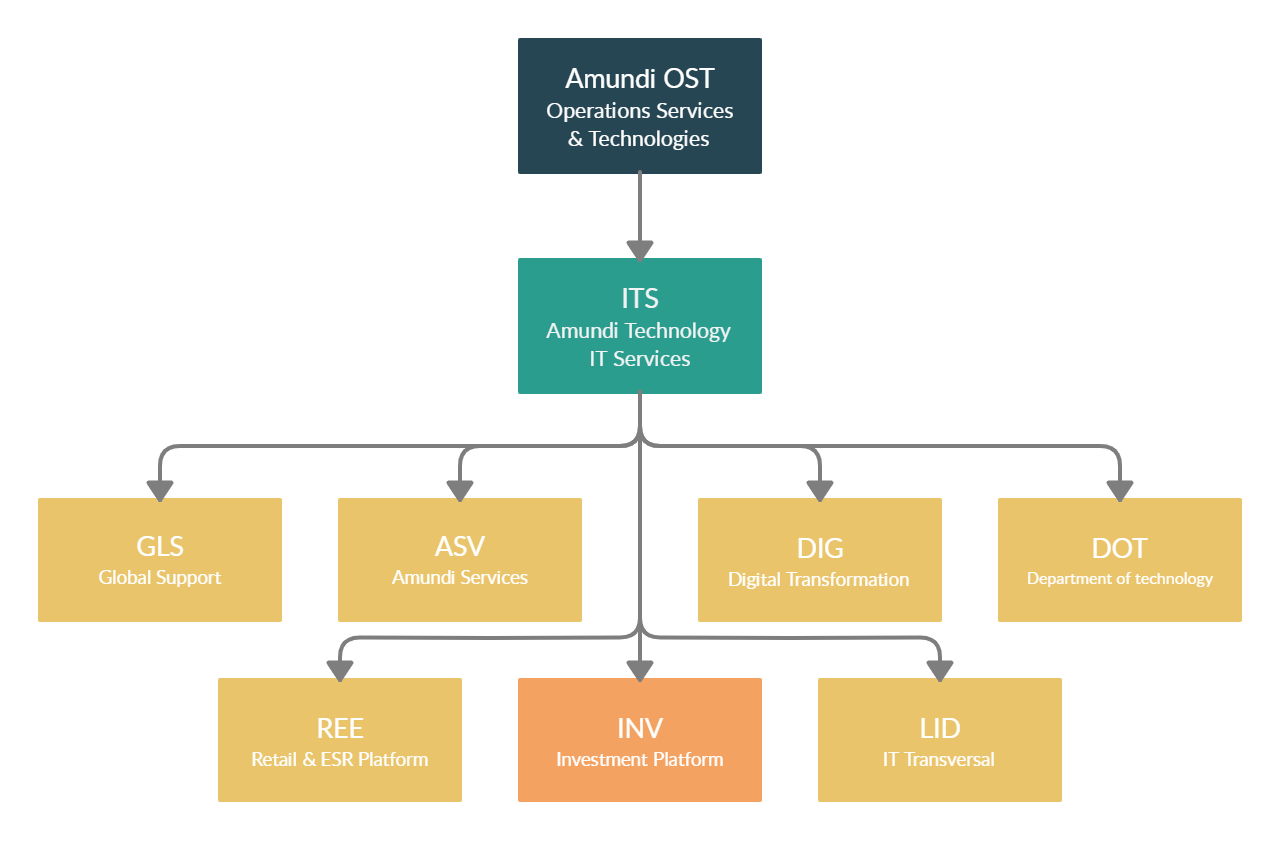
\includegraphics[width=\columnwidth]{img/Org ITS.png}
    \caption{Organisation ITS}
\end{figure}

\section{OST: Operations Services \& Technologies}
\par Amundi AM est subdivisée en plusieurs entités, on retrouve notamment les départements relatifs à l'administration de l'entreprise (par exemple le département DGL, présidé par Mr. Perrier Yves, président et directeur général du groupe Amundi), les départements relatifs au relations clients Amundi AM (par exemple INS: Institutional Clients Division, RET: Retail Clients Division \dots)
\begin{figure}[ht]
    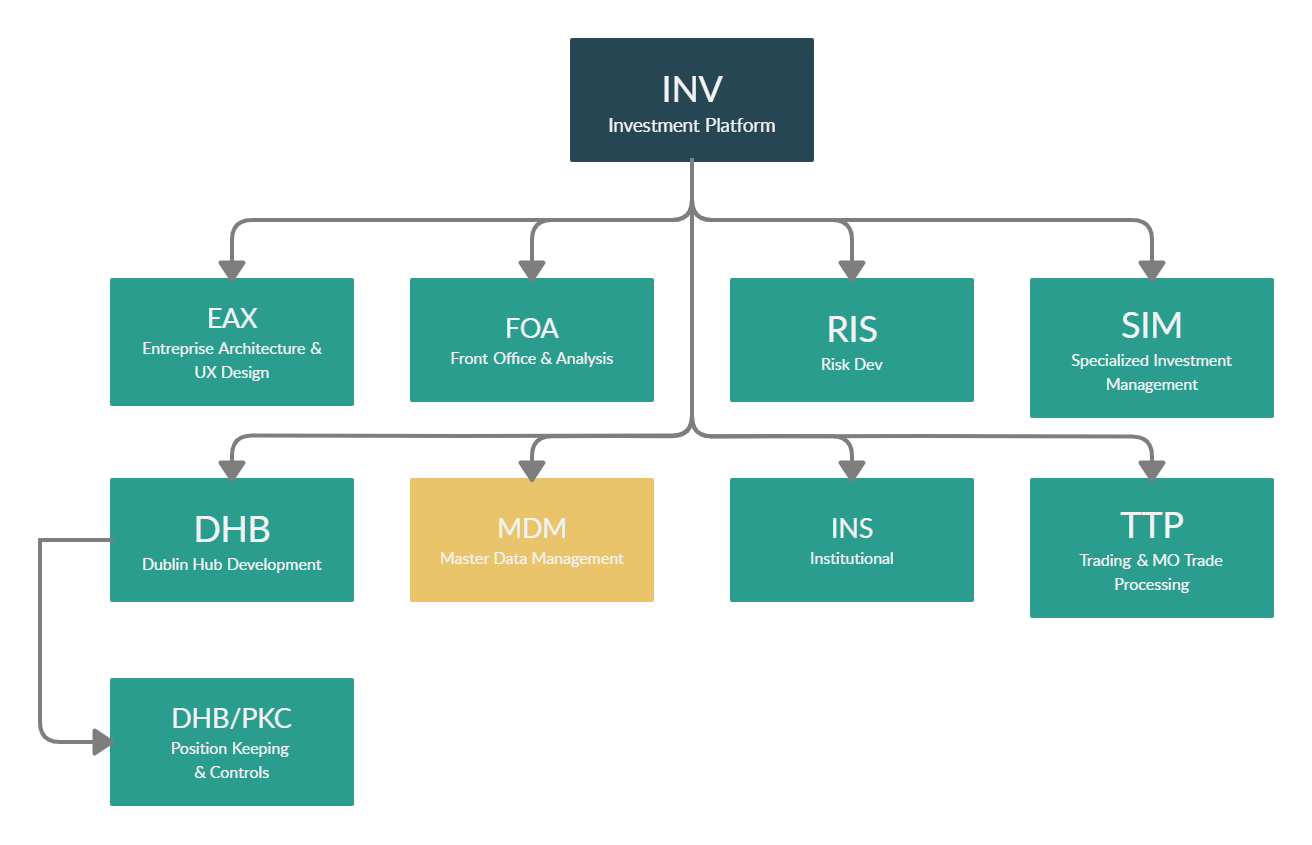
\includegraphics[width=\columnwidth]{img/Org INV.png}
    \caption{Organisation INV}
\end{figure}